%%%%%%%%%%%%%%%%%%%%%%%%%%%%%%%%%%%%%%%%%%%%%%%%%%%%%%%%%%%%%%%%%%%%%%%%%%%%%%%%%%%%%%%%
\section{ordered particle systems} \hspace{1pt}
\label{sec:_ops}
\cite{Forster2005,Forster2011,Forster2010}

\begin{figure}[htb]
\begin{center}
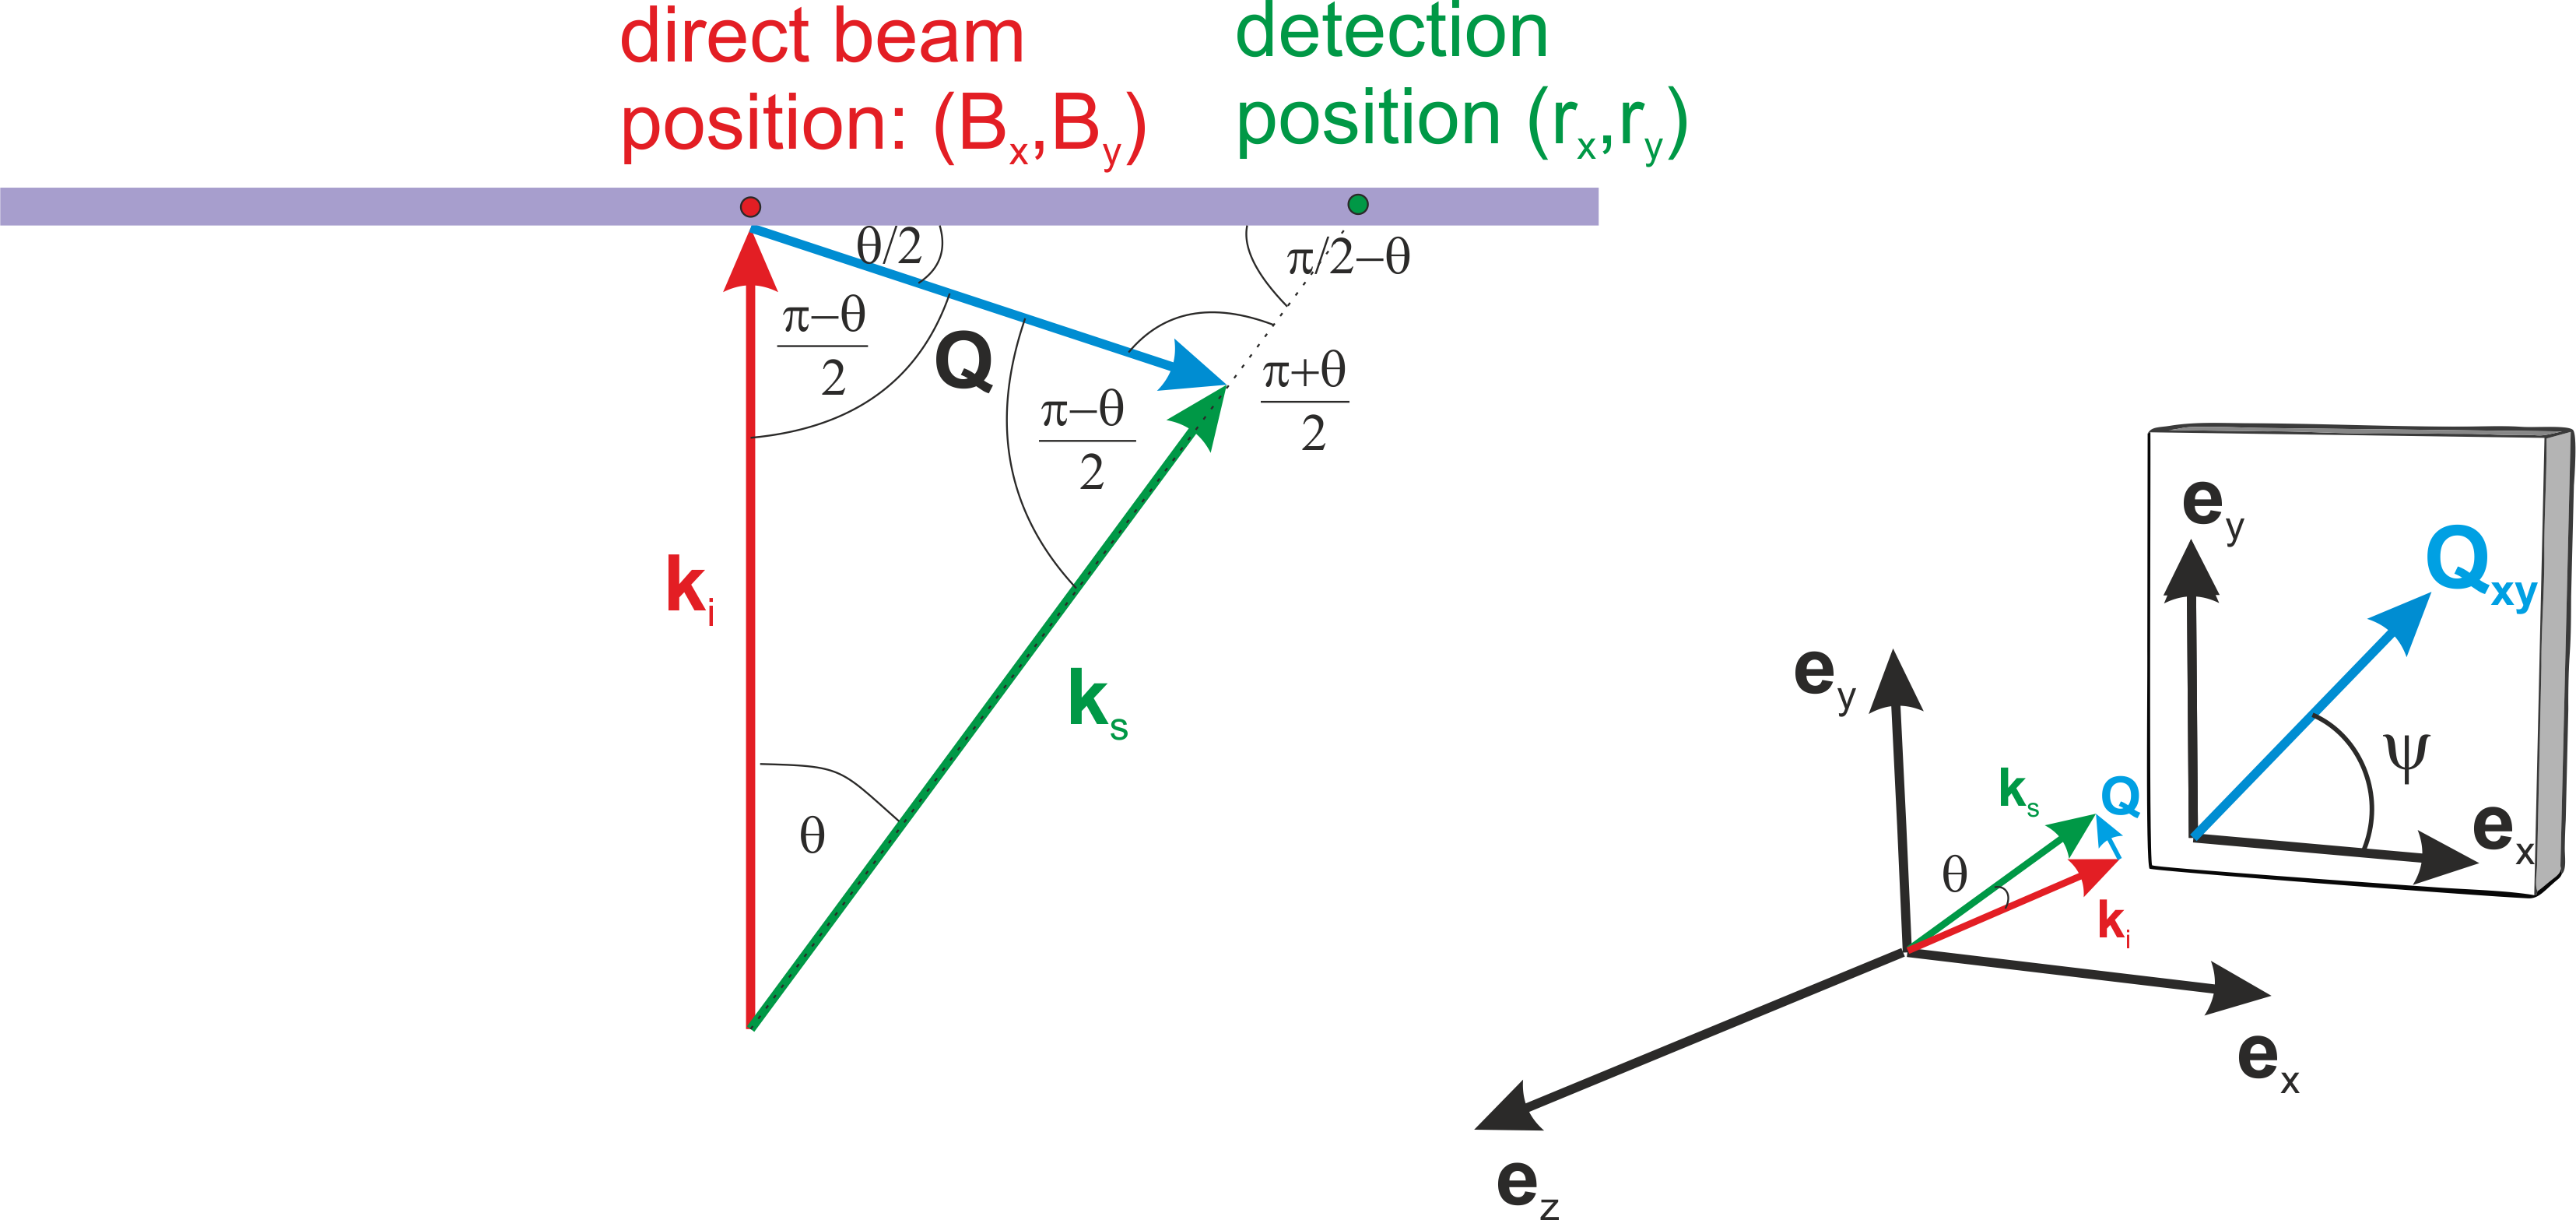
\includegraphics[width=0.85\textwidth]{osp_coord_system.png}
\end{center}
\caption{The scattering vector in polar coordinates coordination system with respect to a laboratory-fixed coordinate system based on the three orthogonal unit vectors ($\mathbf{e}_x$, $\mathbf{e}_y$, $\mathbf{e}_z$). They are arranged such that the x-direction coincides with the x-direction of the detector, and the y-direction coincides with the y-direction of the detector. The direction of the incoming neutron beam is chosen to be $-\mathbf{e}_z$. } \label{fig:opsCoordSys}
\end{figure}

\begin{align}
\mathbf{k}_i &= 
    \left(
        \begin{array}{c}
                  k_{i,x} \\
                  k_{i,y} \\
                  k_{i,z} 
        \end{array}
    \right) 
    = \frac{2\pi}{\lambda}
    \left(
        \begin{array}{c}
                  0\\
                  0 \\
                  -1
        \end{array}
    \right) \\
\mathbf{k}_s &=
    \left(
        \begin{array}{c}
                  k_{i,x} \\
                  k_{i,y} \\
                  k_{i,z}
        \end{array}
    \right)
    = \frac{2\pi}{\lambda}
    \left(
        \begin{array}{c}
                  \cos(\psi) \sin(\theta)\\
                  \sin(\psi) \sin(\theta) \\
                  -\cos(\theta)
        \end{array}
    \right) \\
\mathbf{Q} &= \mathbf{k}_s - \mathbf{k}_i =
    \left(
        \begin{array}{c}
                  Q_{x} \\
                  Q_{y} \\
                  Q_{z}
        \end{array}
    \right)
    = \frac{2\pi}{\lambda}
    \left(
        \begin{array}{c}
                  \cos(\psi) \sin(\theta)\\
                  \sin(\psi) \sin(\theta) \\
                  1-\cos(\theta)
        \end{array}
    \right)
\end{align}